% sections/01_simulation.tex: generated by newdeck/html2beamer.py from the HTML deck, then edited by hand

% ---------------------------------------------------------------- slide 6: Outline
\begin{btframe}{}{Outline}
\begin{outlinelist}
\outlineitem{1}{Introduction}{the background types, the geometry, the input muons and neutrinos}{0.35}
\outlineitem{2}{Simulation}{transport, inelastic scattering, technologies, hits and digitisation, signal generation}{1.00}
\outlineitem{3}{Selection}{track cuts, pair cuts and time coincidence}{0.35}
\outlineitem{4}{Backgrounds before tagging}{μ and ν inelastic scattering, MS7 K\textsubscript{L}, combinatorial pairs}{0.35}
\outlineitem{5}{Background tagging}{rules, V0 rule, SBT model, R1, R2, summary}{0.35}
\outlineitem{6}{Optimisation and conclusion}{genetic-algorithm search, the optimised designs Z2 and Z3}{0.35}
\end{outlinelist}
\end{btframe}

% ---------------------------------------------------------------- slide 7: Transport through the shield and the cavern: Cuda Muons
\begin{btframe}{2 · Simulation · transport}{Transport through the shield and the cavern: Cuda Muons}
{\centering 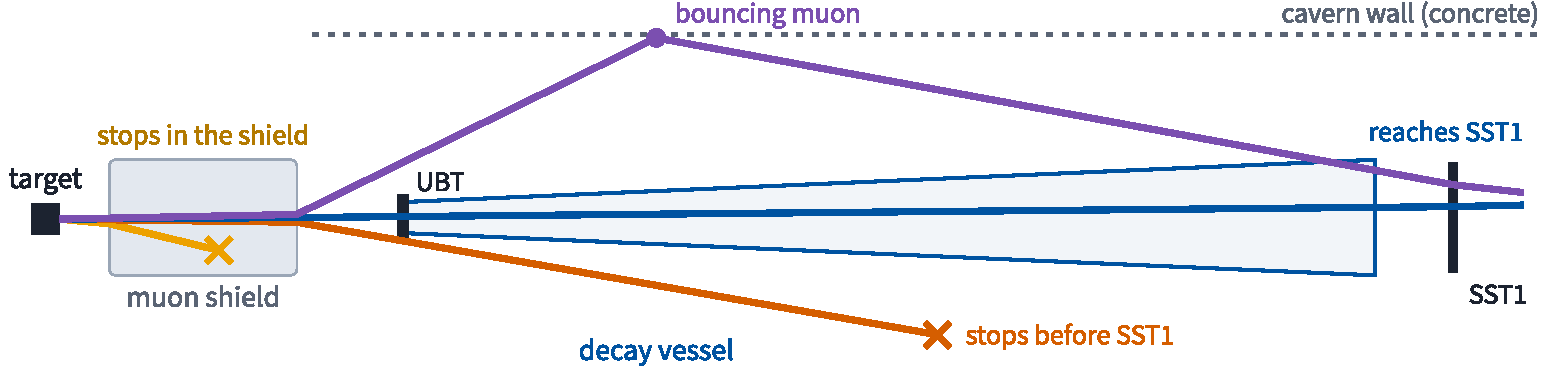
\includegraphics[width=1.00\linewidth,height=59.18pt,keepaspectratio]{figs/s06_sk1.pdf}\par}
\vspace{2.46pt}
\noindent \begin{minipage}[t]{\dimexpr(0.4651\linewidth-0.4651\dimexpr11.49pt\relax)}\vspace{0pt}\raggedright
{\centering 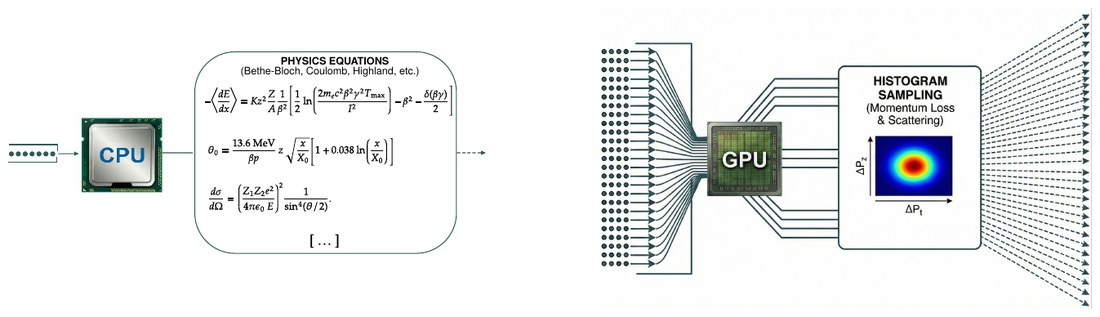
\includegraphics[width=1.00\linewidth,keepaspectratio]{figs/s06_img2.jpg}\par}
{\color{muted}\fontsize{5.48pt}{8.71pt}\selectfont Geant4 on a CPU, one muon at a time (left) vs Cuda Muons on a GPU (right)\par}
\vspace{2.46pt}
% {\centering 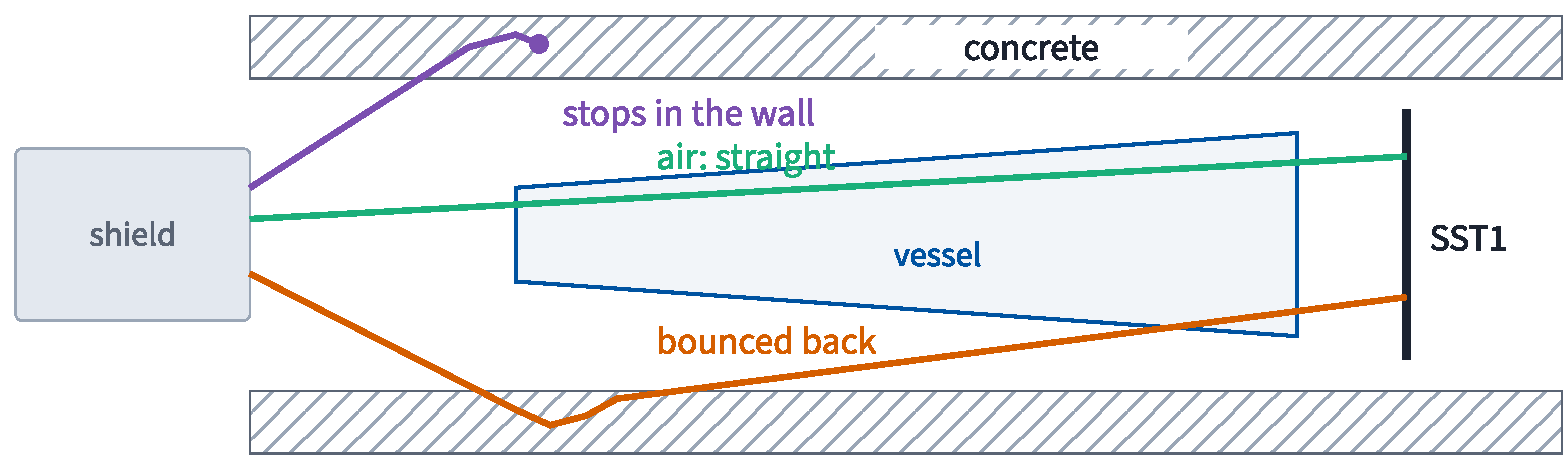
\includegraphics[width=1.00\linewidth,height=54.62pt,keepaspectratio]{figs/s06_sk3.pdf}\par}
\end{minipage}%
\hfill%
\begin{minipage}[t]{\dimexpr(0.5349\linewidth-0.5349\dimexpr11.49pt\relax)}\vspace{0pt}\raggedright
{\fontsize{5.92pt}{8.03pt}\selectfont
\begin{itemize}
  \item[\status{blue}] Offline: Geant4 fills per-material histograms of momentum loss and p\textsubscript{T} kick for a fixed 2 cm step (95 log bins, 0.18–400 GeV)
  \item[\status{blue}] Online: one CUDA thread per muon samples them in O(1) (alias method); field integrated with RK4
    \item[\status{blue}] Nov-4 production (Shah Rukh): the Nov-4 target pool transported through the TRY6 shield and the cavern 3 220 times, one seed = one spill
    \item[\status{blue}] Stored: each muon’s state @UBT and @SST1
  \item[\status{green}] One GPU: >10\textsuperscript{4}× faster than single-core Geant4, >100× faster than 1024 CPU cores
  \item[\status{red}] Decays are not simulated
  \item[\status{red}] Air is not simulated: muons travel in straight lines through the cavern air

\end{itemize}}
\end{minipage}\par
\slidenote{L. F. P. Cattelan, S. R. Qasim, P. H. Owen, N. Serra, “Ultra-Fast Muon Transport via Histogram Sampling on GPUs”, arXiv:2512.10520 (2025).}
\end{btframe}

% ---------------------------------------------------------------- slide 8: How an inelastic interaction is made: seven steps
\begin{btframe}{2 · Simulation · inelastic scattering}{How an inelastic interaction is made: seven steps}
\begin{flowrow}{\dimexpr(\linewidth-6\dimexpr6.37pt\relax)/7\relax}{6.37pt}%
\flowstep{white}{rule}{2.28pt}{3.64pt}{{\fontsize{5.92pt}{7.40pt}\selectfont\textbf{\textcolor{cern}{1 · parents}}\par}\vspace{0.91pt}{\fontsize{5.01pt}{6.76pt}\selectfont\textcolor{ink}{muons from the Nov-4 transport, ν from the 2026 flux, straight through each target}\par}}%
\flowarrow%
\flowstep{white}{rule}{2.28pt}{3.64pt}{{\fontsize{5.92pt}{7.40pt}\selectfont\textbf{\textcolor{cern}{2 · cross section}}\par}\vspace{0.91pt}{\fontsize{5.01pt}{6.76pt}\selectfont\textcolor{ink}{Kokoulin per nucleon (μ), GENIE splines (ν)}\par}}%
\flowarrow%
\flowstep{white}{rule}{2.28pt}{3.64pt}{{\fontsize{5.92pt}{7.40pt}\selectfont\textbf{\textcolor{cern}{3 · forced}}\par}\vspace{0.91pt}{\fontsize{5.01pt}{6.76pt}\selectfont\textcolor{ink}{one interaction per crossing, weight w·P = interactions per spill}\par}}%
\flowarrow%
\flowstep{white}{rule}{2.28pt}{3.64pt}{{\fontsize{5.92pt}{7.40pt}\selectfont\textbf{\textcolor{cern}{4 · generator}}\par}\vspace{0.91pt}{\fontsize{5.01pt}{6.76pt}\selectfont\textcolor{ink}{Geant4 muonNuclear + Pythia 6 (μ), GENIE 3.06 (ν)}\par}}%
\flowarrow%
\flowstep{white}{rule}{2.28pt}{3.64pt}{{\fontsize{5.92pt}{7.40pt}\selectfont\textbf{\textcolor{cern}{5 · short-lived}}\par}\vspace{0.91pt}{\fontsize{5.01pt}{6.76pt}\selectfont\textcolor{ink}{K\textsubscript{S}, Λ, π\textsuperscript{0} … decayed; in MS7 handed to Geant4}\par}}%
\flowarrow%
\flowstep{white}{rule}{2.28pt}{3.64pt}{{\fontsize{5.92pt}{7.40pt}\selectfont\textbf{\textcolor{cern}{6 · transport}}\par}\vspace{0.91pt}{\fontsize{5.01pt}{6.76pt}\selectfont\textcolor{ink}{straight to SST1 with scattering (vessel); Geant4 + field map through the MS7 iron}\par}}%
\flowarrow%
\flowstep{white}{rule}{2.28pt}{3.64pt}{{\fontsize{5.92pt}{7.40pt}\selectfont\textbf{\textcolor{cern}{7 · selection, tagging}}\par}\vspace{0.91pt}{\fontsize{5.01pt}{6.76pt}\selectfont\textcolor{ink}{as for the muon pairs; own and random hits}\par}}%
\end{flowrow}
\vspace{2.46pt}
\noindent \begin{minipage}[[c]{0.5\linewidth}
{\fontsize{4.55pt}{6.15pt}\selectfont \textcolor{cern}{\textbf{2 · cross section: μ, per nucleon in iron}}\par}
\vspace{0.55pt}
{\centering 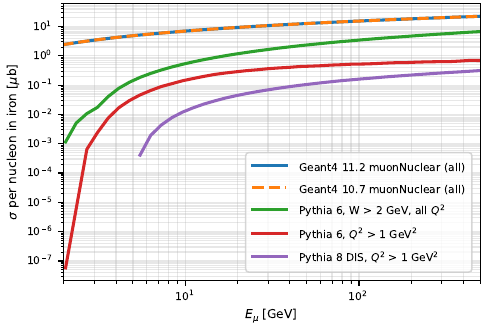
\includegraphics[height=86.49pt,keepaspectratio]{figs/s07_img1.png}\par}
\end{minipage}%
\hfill%
\begin{minipage}[c]{0.5\linewidth}
{\fontsize{4.55pt}{6.15pt}\selectfont \textcolor{cern}{\textbf{2 · cross section: ν, σ/E per nucleon on \textsuperscript{56}Fe}}\par}
\vspace{0.55pt}
{\centering 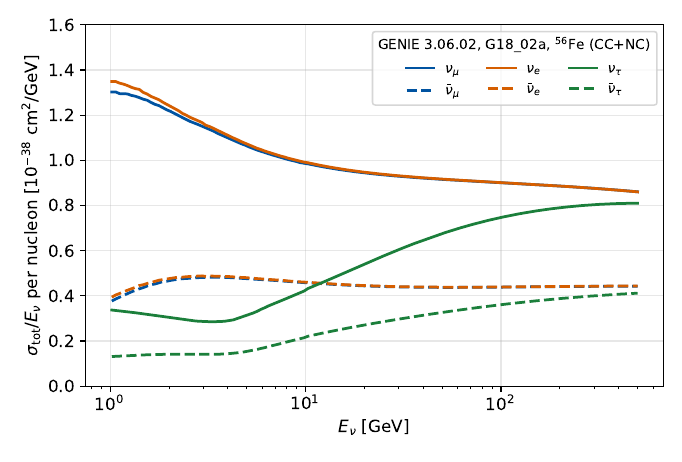
\includegraphics[height=86.49pt,keepaspectratio]{figs/s07_img2.png}\par}
\end{minipage}%
\hfill%
\vspace{2.46pt}
{\fontsize{4.55pt}{6.15pt}\selectfont \centering \textcolor{cern}{\textbf{3 · forced interaction}}\par}
\vspace{0.82pt}
{\centering 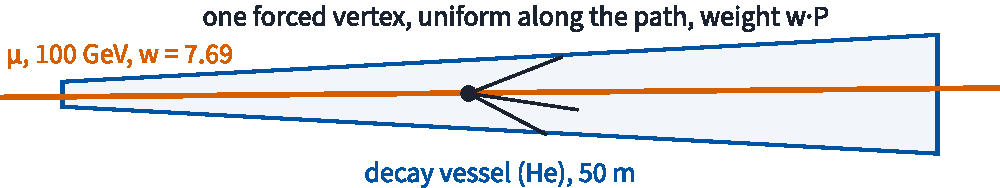
\includegraphics[width=1.00\linewidth,height=29.59pt,keepaspectratio]{figs/s07_sk3.pdf}\par}
\vspace{0.82pt}
{\fontsize{4.78pt}{6.45pt}\selectfont \centering P = n σ L along the crossing (helium, 10 GeV: 4×10\textsuperscript{-6}); the vertex is forced, the event weight w·P = interactions per spill\par}

\end{btframe}

% ---------------------------------------------------------------- slide 9: Detector technologies and the cost unit: the drachma
\begin{btframe}{2 · Simulation · technologies}{Detector technologies and the cost unit: the drachma}
{\fontsize{6.36pt}{8.66pt}\selectfont\setlength{\tabcolsep}{3.05pt}\renewcommand{\arraystretch}{1.42}
\begin{tabularx}{\linewidth}{>{\raggedright\arraybackslash}Xrrrr}
\textcolor{muted}{} & \textcolor{muted}{straw (UBT)} & \textcolor{muted}{tile} & \textcolor{muted}{tile2 (flames)} & \textcolor{muted}{LS + WOM (SBT)} \\\headrule
layers & 6 (vertical) & 1 & 1 & LS cell 20 cm \\\rowrule
cell & 5 mm & 4 × 4 cm\textsuperscript{2} & 2 × 2 cm\textsuperscript{2} & 80 × ≤150 cm\textsuperscript{2} \\\rowrule
σ\textsubscript{t} / window & drift, ±25 ns & 120 ps, ±3σ & 90 ps, ±3σ & \textasciitilde{}1 ns, ±3 ns \\\rowrule
efficiency & 99.9 \% & 99.9 \% & 99.9 \% & 99.3 \% \\\rowrule
X / X\textsubscript{0} & 0.12 \% & 2.4 \% & 2.4 \% & \textasciitilde{}40 \% \\\rowrule
cost / m\textsuperscript{2} (drachmas) & 2.9 & 4.0 & 16.9 & \textasciitilde{}0.34 \\\rowrule
\end{tabularx}\par}

\vspace{2.46pt}
\noindent
\begin{minipage}[c]{0.6\linewidth}
    \raggedright
    {\fontsize{6.15pt}{8.30pt}\selectfont
    \textcolor{cern}{\textbf{R2 = 333.5 drachmas = the budget
    \textcolor{muted}{{\fontsize{4.61pt}{5.99pt}\selectfont
    (R1 99.7)}}}}\par}
    \vspace{2.46pt}
    {\centering
    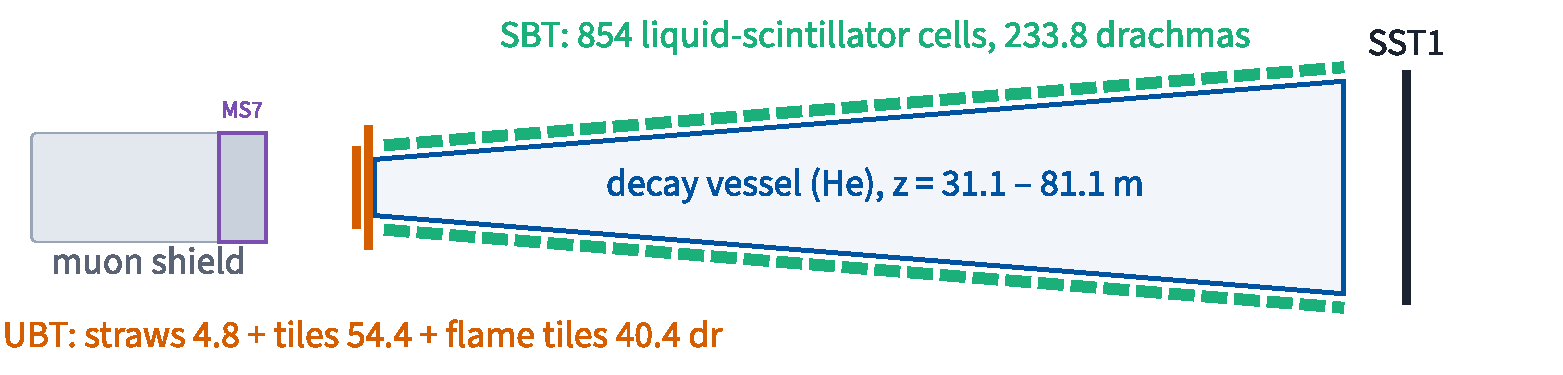
\includegraphics[width=\linewidth,keepaspectratio]
    {figs/s08_sk3.pdf}\par}
\end{minipage}%
\hfill
\begin{minipage}[c]{0.125\linewidth}
    \centering
    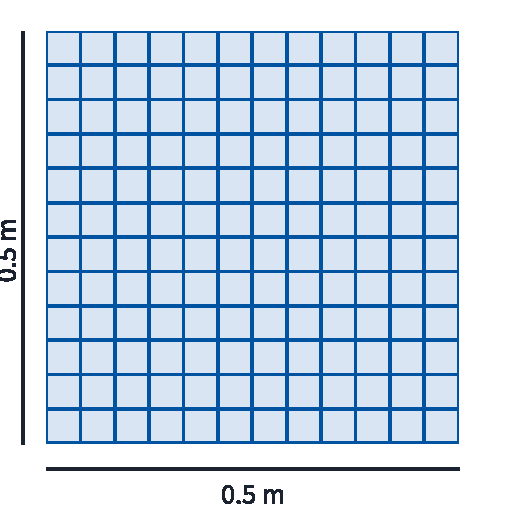
\includegraphics[width=\linewidth,keepaspectratio]
    {figs/s08_sk1.pdf}
\end{minipage}%
\hfill
\begin{minipage}[c]{0.04\linewidth}
    \centering
    {\fontsize{13.66pt}{18.44pt}\selectfont
    \textcolor{cern}{\textbf{=}}}
\end{minipage}%
\hfill
\begin{minipage}[c]{0.145\linewidth}
    \centering
    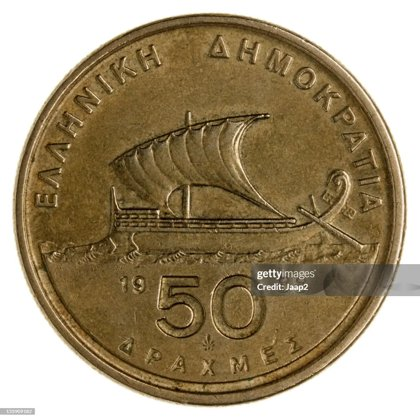
\includegraphics[width=\linewidth,keepaspectratio]
    {figs/s08_img2.jpg}
\end{minipage}%
\par
% \hfill%
\vspace{2.46pt}
\noindent 
% \begin{minipage}[c]{\dimexpr(0.2500\linewidth-0.2500\dimexpr16.96pt\relax)}\raggedright
{\fontsize{6.02pt}{8.43pt}\selectfont
\begin{itemize}
  \item \textbf{1 drachma} = the cost of one 0.5 × 0.5 m\textsuperscript{2} module of 4 × 4 cm\textsuperscript{2} tiles (144 tiles)
  \item Relative costs from one placeholder model: channels × relative cost per channel + 10 \% mechanics; never absolute money
\end{itemize}}
% \end{minipage}\par

\end{btframe}


% ---------------------------------------------------------------- slide 10: Hits and digitisation: own hits, random hits, time windows
\begin{btframe}{2 · Simulation · hits and digitisation}{Hits and digitisation: own hits, random hits, time windows}
{\fontsize{6.02pt}{7.52pt}\selectfont\setlength{\tabcolsep}{3.51pt}\renewcommand{\arraystretch}{1.42}
\begin{tabularx}{\linewidth}{lrr>{\raggedright\arraybackslash}Xr}
\textcolor{muted}{plane} & \textcolor{muted}{cell} & \textcolor{muted}{time window} & \textcolor{muted}{position} & \textcolor{muted}{efficiency} \\\headrule
UBT straws & 6 layers, vertical, 5 mm & 50 ns drift: ±25 ns & no position along the 0.9 m section & 99.9 \% \\\rowrule
UBT tiles & 4 × 4 cm\textsuperscript{2} (2 × 2 cm\textsuperscript{2} in the flames) & ±3σ (σ 120 / 90 ps) & cell centre & 99.9 \% \\\rowrule
SBT cells & 854 LS cells, 20 cm, 30 MeV threshold & \textasciitilde{}1 ns, ±3 ns & cell + pointing along the wall & 99.3 \% \\\rowrule
\end{tabularx}\par}
\vspace{2.46pt}
\noindent \begin{minipage}[c]{0.5\linewidth}
{\centering 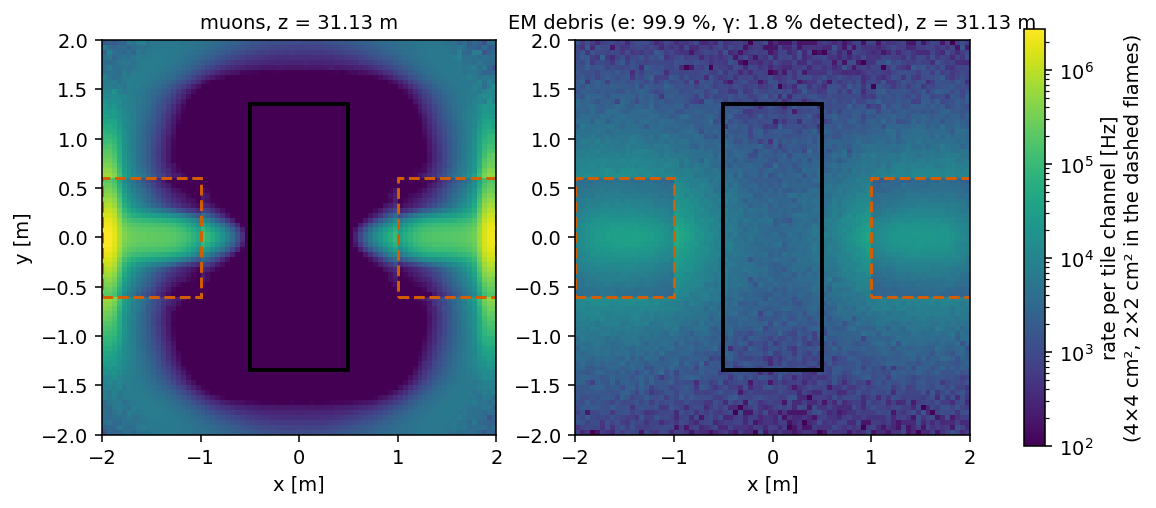
\includegraphics[width=1\linewidth,keepaspectratio]{figs/s09_img1.png}\par}
\end{minipage}%
\hfill%
\begin{minipage}[c]{0.5\linewidth}
{\fontsize{6.02pt}{8.43pt}\selectfont
\begin{itemize}
  \item \textbf{Own hits:} each simulated particle is crossed with every plane; a hit if the cell fires (efficiency, threshold, energy deposit in the LS)
  \item \textbf{Random hits:} all the other muons of the spill, Poisson from full-statistics rate maps, 
  \begin{equation*}
      \langle N_\text{acc}\rangle  = R_\text{plane} · 2W / 1 s
  \end{equation*}
  \item \textbf{EM debris} of the shield end (e / γ) added to the UBT rate maps
  \item \textbf{Scattering} in the vessel walls and the SBT shell, mean \textbf{energy loss} in the shell (soft muons stop)
  \item A track is \textbf{tagged} by a hit in its space–time window on any plane upstream of its vertex
  \item Tile plane: up to 2.8 MHz per channel from muons in the flames, ≤ 53 kHz from EM debris; mean random hits per tile in ±0.36 ns: 2×10\textsuperscript{-3} (μ), 4×10\textsuperscript{-5} (EM)
\end{itemize}}
\end{minipage}\par
\slidenote{$N_\text{acc}$ is the mean number of accidental hits. The actual number is drawn from a Poisson distribution with that mean, independently for each event. $R_\text{plane}$ the total rate of hits on the whole plane, The maps are built from the full muon sample, EM debris included, and the SBT uses ×4 itssimulated rate.  - 2W: the full width of the time window the plane is read in. W is the half-width; for    tiles the window is ±1.5 ns, so 2W = 3 ns.}
\end{btframe}

% ---------------------------------------------------------------- slide 11: Signal: truth-level generation with EventCalc
\begin{btframe}{2 · Simulation · signal}{Signal: truth-level generation with EventCalc}
\begin{flowrow}{\dimexpr(\linewidth-3\dimexpr6.37pt\relax)/4\relax}{6.37pt}%
\flowstep{white}{rule}{2.28pt}{3.64pt}{{\fontsize{5.92pt}{7.40pt}\selectfont\textbf{\textcolor{cern}{production}}\par}\vspace{0.91pt}{\fontsize{5.91}{6.76pt}\selectfont\textcolor{ink}{tabulated P(θ, E) per proton;\\ LLP from the target centre, straight}\par}}%
\flowarrow%
\flowstep{white}{rule}{2.28pt}{3.64pt}{{\fontsize{5.92pt}{7.40pt}\selectfont\textbf{\textcolor{cern}{decay vertex}}\par}\vspace{0.91pt}{\fontsize{5.91}{6.76pt}\selectfont\textcolor{ink}{exponential in the decay volume, weight P\textsubscript{decay}}\par}}%
\flowarrow%
\flowstep{white}{rule}{2.28pt}{3.64pt}{{\fontsize{5.92pt}{7.40pt}\selectfont\textbf{\textcolor{cern}{decay}}\par}\vspace{0.91pt}{\fontsize{5.91}{6.76pt}\selectfont\textcolor{ink}{all channels of the model (423 blocks), Pythia for the hadrons}\par}}%
\flowarrow%
\flowstep{white}{rule}{2.28pt}{3.64pt}{{\fontsize{5.92pt}{7.40pt}\selectfont\textbf{\textcolor{cern}{to tracks}}\par}\vspace{0.91pt}{\fontsize{5.91}{6.76pt}\selectfont\textcolor{ink}{daughters through field and matter to SST1 and the TD, then the same selection}\par}}%
\end{flowrow}
\vspace{2.46pt}
\noindent \begin{minipage}[c]{0.5\linewidth}
{\fontsize{6.11pt}{6.34pt}\selectfont\setlength{\tabcolsep}{2.88pt}\renewcommand{\arraystretch}{1.42}
\begin{tabular}{llr}
\textcolor{muted}{model} & \textcolor{muted}{coupling} & \textcolor{muted}{masses [GeV]} \\\headrule
HNL & pure e mixing; pure μ mixing & 0.5, 1, 2, 3, 4 \\\rowrule
dark photon & kinetic mixing, primary + cascade production & 0.3, 0.9, 2, 4 \\\rowrule
Higgs-like scalar & mixing with the Higgs & 0.5, 1, 2, 4 \\\rowrule
ALP & coupling to fermions & 0.5, 1, 2, 4 \\\rowrule
\end{tabular}\par}
\end{minipage}%
\hfill%
\begin{minipage}[c]{0.5\linewidth}
{\fontsize{6.11pt}{6.34pt}\selectfont\setlength{\tabcolsep}{2.88pt}\renewcommand{\arraystretch}{1.42}
\begin{tabularx}{\linewidth}{l>{\raggedright\arraybackslash}Xr}
\textcolor{muted}{model} & \textcolor{muted}{two-body} & \textcolor{muted}{three-body (missing ν / π\textsuperscript{0})} \\\headrule
HNL & N → π\textsuperscript{±} ℓ\textsuperscript{\ensuremath{\mp}} (full) & N → ℓ\textsuperscript{+} ℓ\textsuperscript{−} ν (partial) \\\rowrule
dark photon & A′ → μ\textsuperscript{+} μ\textsuperscript{−}, e\textsuperscript{+} e\textsuperscript{−} (full) & A′ → π\textsuperscript{+} π\textsuperscript{−} π\textsuperscript{0} (partial) \\\rowrule
scalar & S → π\textsuperscript{+} π\textsuperscript{−}, K\textsuperscript{+} K\textsuperscript{−}, μ\textsuperscript{+} μ\textsuperscript{−} (full) & – \\\rowrule
ALP & a → μ\textsuperscript{+} μ\textsuperscript{−} (full) & a → π\textsuperscript{+} π\textsuperscript{−} π\textsuperscript{0}, η π π (partial) \\\rowrule
\end{tabularx}\par}
\end{minipage}\par
\vspace{2.46pt}
{\centering {\centering 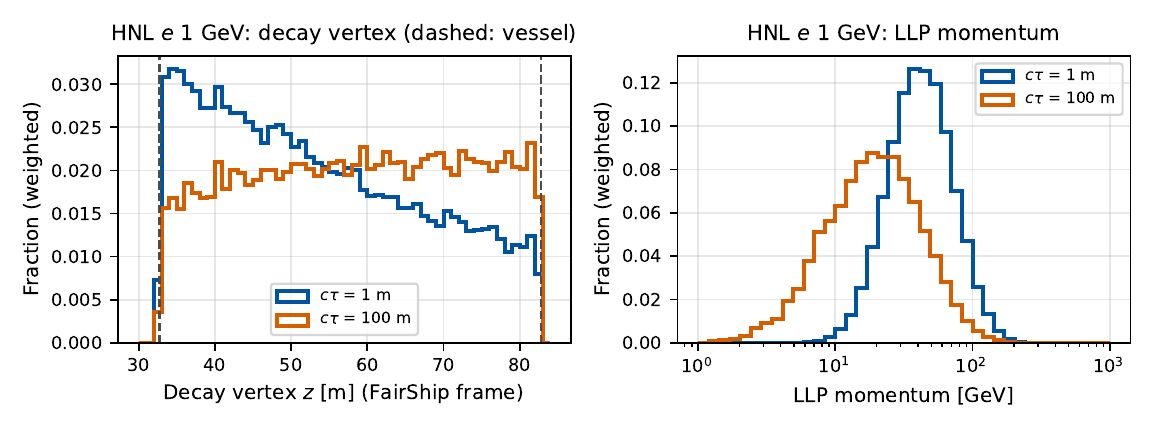
\includegraphics[height=109.04pt,keepaspectratio]{figs/s10_img1.png}\par}
\noindent
{\fontsize{6.78pt}{7.45pt}\selectfont cτ = 1 m and 100 m; 5×10\textsuperscript{4} LLPs per point, 3–4.5×10\textsuperscript{4} decaying in the vessel; efficiencies P\textsubscript{decay}-weighted\par}
\par}
\end{btframe}
